\section{Potenzfunktionen}\label{sec:Potenzfunktionen}
\subsection{Definition}\label{sec:Potenzfunktionen/Definition}
Betrachtet man eine Funktion $f(x)=x^n$, wobei $n\in\mathbb{N}\setminus\{0\}$, so spricht man von einer Potenzfunktion. Der Begriff `{}Potenzfunktion`{} ist hierbei ein Schirmbegriff für alle Funktionen, die eine Potenz besitzen. Im Folgenden unterscheidet man zwischen
\begin{itemize}
	\item $n>0$ und $ n\equiv0$ $(\mathrm{mod}2)$ Bedeutet, dass $n$ größer als 0 ist und einen kongruenten Modulo hat für den Modulo aus 2 und den Wert $0$. Wird $n$ geteilt durch $2$, so muss der Modulo $0$ ergeben.
	\item $n>0$ und $ n\equiv1$ $(\mathrm{mod}2)$
	\item $n<0$ und $ n\equiv0 $ $(\mathrm{mod}2)$
	\item $n<0$ und $ n\equiv1$ $(\mathrm{mod}2)$
\end{itemize}
\subsection{Potenzfunktionen mit $n>0$}\label{sec:Potenzfunktionen/Potenzfunktionen mit positivem Exponenten}
Bei Potenzfunktionen unterscheidet man im wesentlichen zwischen $n>0$ und $n<0$ und zwischen geraden und ungeraden Exponenten
\subsubsection{Potentfunktion mit $n>0 $ und $ n\equiv0$ $(\mathrm{mod}2)$}
Ist $n$ gerade und positiv, so hat eine Funktion $f(x)=x	^n$ folgende Eigenschaften.
\begin{itemize}
	\item Der Graph ist Achsensymmetrisch zu der $Y$-Achse
	\item Der Graph verläuft parabolisch
	\item Für $x<0$ steigt der Graph
	\item Für $x>0$ steigt der Graph
	\item Je höher der Exponent, desto flacher verläuft der Graph für $-1<x>1$ und desto steiler für $x>1$ und $x<-1$
\end{itemize}
\begin{figure}[h!]
\centering
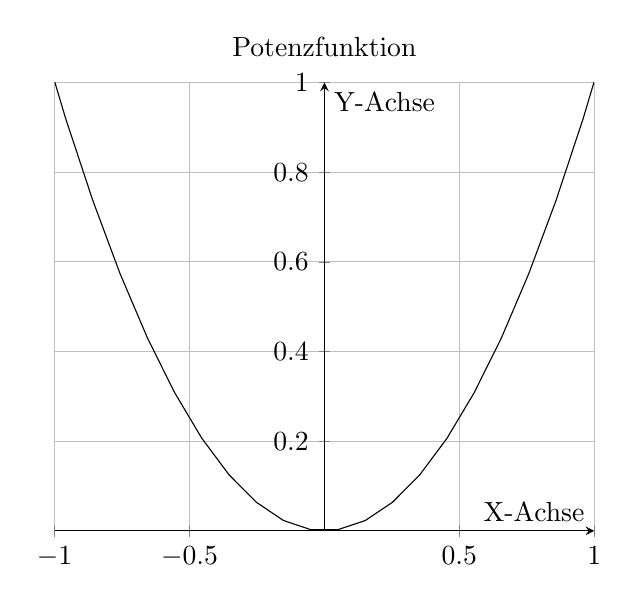
\begin{tikzpicture}
\begin{axis}[
    title={Potenzfunktion},
    xlabel={X-Achse},
    ylabel={Y-Achse},
    axis lines=middle, % Zentriert die Achsen
    xmin=-1, xmax=1, % Setzt die Grenzen für die X-Achse
    ymin=0, ymax=1, % Setzt die Grenzen für die Y-Achse
    grid=major, % Fügt ein Hauptgitter hinzu
]
\addplot[mark=none, samples=100] {x^2};
\end{axis}
\end{tikzpicture}
\caption{Quadratische Funktion mit $n>0$ und $ n\equiv0$ $(\mathrm{mod}2)$}
\end{figure}
\geogebra{https://www.geogebra.org/m/cand2jpf}
\subsubsection{Potenzfunktion mit $n>0$ und $ n\equiv1$ $(\mathrm{mod}2)$}
Ist $n>0$ und ungerade, so hat $f(x)=x^n$ die folgenden Eigenschaften.
\begin{itemize}
	\item $f(x)$ ist punktsymmetrisch zum Ursprung
	\item $f(x)$ verläuft von links nach rechts (vom 1. Quadranten zum 3. Quadranten), dies bedeutet die Form ist kubisch. %TODO Quadranten Blatt hinzufügen
	\item Je größer der Exponent ist, desto flacher verläuft $f$ für $-1<x<1$ und steiler für $x>1$ bzw. $x<-1$
	\item Die Funktion, die die geben Eigenschaften erfüllen sind alle monoton steigend
\end{itemize}
\begin{figure}[h!]
\centering
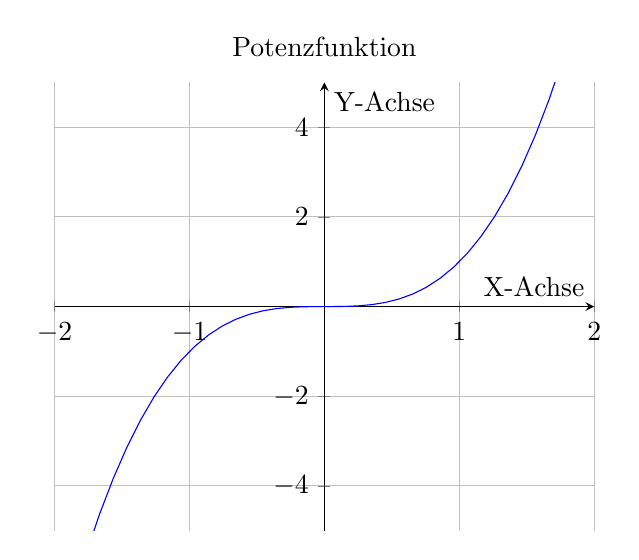
\begin{tikzpicture}
\begin{axis}[
    title={Potenzfunktion},
    xlabel={X-Achse},
    ylabel={Y-Achse},
    axis lines=middle, % Zentriert die Achsen
    xmin=-2, xmax=2, % Setzt die Grenzen für die X-Achse
    ymin=-5, ymax=5, % Setzt die Grenzen für die Y-Achse
    grid=major, % Fügt ein Hauptgitter hinzu
]
\addplot+[mark=none, samples=100]{x^3};
\end{axis}
\end{tikzpicture}
\caption{Potenzfunktion mit $n>0$ und $ n\equiv1$ $(\mathrm{mod}2)$}
\end{figure}
\subsection{Potenzfunktion mit $n<0$ - Hyperbel}\label{sec:Potenzfunktionen/Potenzfunktionen mit negativem Exponenten}
Hat eine Funktion $f(x)=x^n$ einen negativen Exponenten, so bezeichnet man die Funktion als Hyperbel. Hyperbeln haben eine Definitionslücke, dass heißt, es gibt Zahlen, die man nicht für $x$ einsetzten darf. Hyperbeln verlaufen asymptotisch, dass heißt, es existieren Geraden, deren sich der Graph unendlich nah annähert, diese allerdings nicht tangiert. Besitzen sie einen geraden Exponenten verlaufen sie Achsensymmetrisch. Ist der Exponent ungerade, so verläuft der Graph punktsymmetrisch. 
\subsubsection{Potenzfunktionen mit $n<0$ und $n\equiv0(mod2)$}
Auch wie bei Potenzfunktionen mit einem positiven Exponenten gibt es Eigenschaften, die ein Graph einer Funktion mit einem negativen geraden Exponenten erfüllt.
\begin{itemize}
	\item Der Graph ist achsensymmetrisch
	\item Der Graph verläuft durch den Punkt $(-1;1)$
	\item Der Graph steigt für $x>0$ und fällt für $x<0$
\end{itemize}
\begin{figure}[h!]
\centering
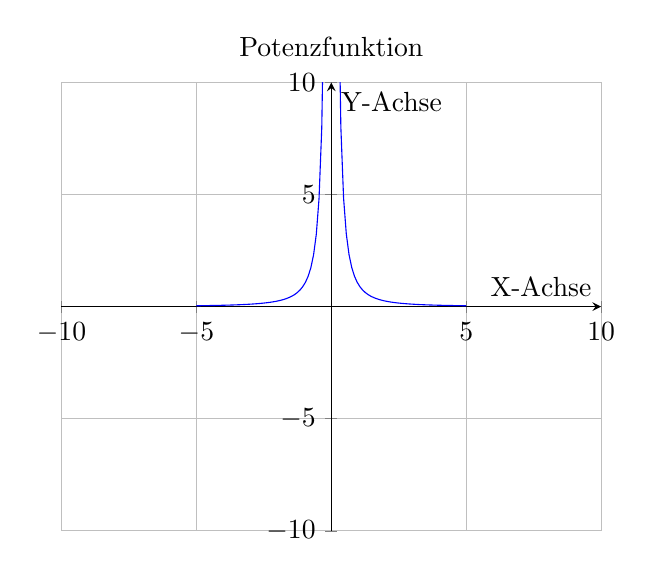
\begin{tikzpicture}
\begin{axis}[
    title={Potenzfunktion},
    xlabel={X-Achse},
    ylabel={Y-Achse},
    axis lines=middle, % Zentriert die Achsen
    xmin=-10, xmax=10, % Setzt die Grenzen für die X-Achse
    ymin=-10, ymax=10, % Setzt die Grenzen für die Y-Achse
    grid=major, % Fügt ein Hauptgitter hinzu
]
\addplot+[mark=none, samples=100]{x^(-2)};
\end{axis}
\end{tikzpicture}
\caption{Potenzfunktion mit $n<0$ und $ n\equiv0$ $(\mathrm{mod}2)$}
\end{figure}
\subsubsection{Potenzfunktionen mit $n<0$ und $n\equiv1(mod2)$}
Die Eigenschaften einer Potenzfunktion mit einem negativen ungeraden Exponenten sind die folgenden. 
\begin{itemize}
	\item Der Graph ist punktsymmetrisch zum Ursprung
	\item Der Graph verläuft durch den Punkt $(-1;1)$
	\item Der Graph fällt für $x>1$ sowohl als auch für $x<0$
\end{itemize}
\begin{figure}[h!]
\centering
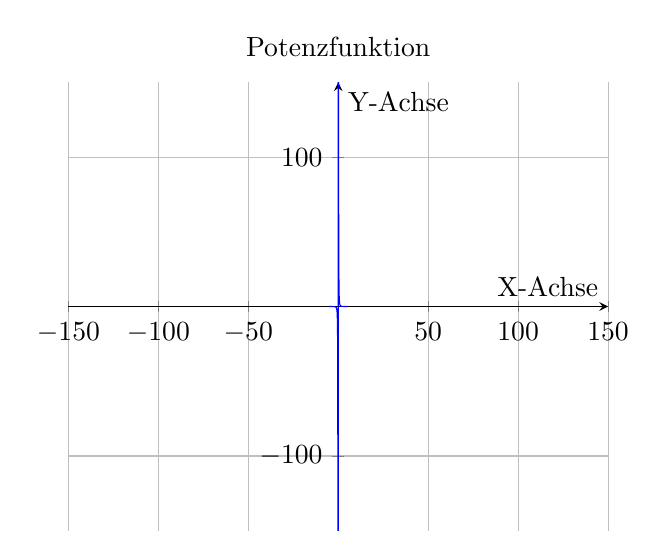
\begin{tikzpicture}
\begin{axis}[
    title={Potenzfunktion},
    xlabel={X-Achse},
    ylabel={Y-Achse},
    axis lines=middle, % Zentriert die Achsen
    xmin=-150, xmax=150, % Setzt die Grenzen für die X-Achse
    ymin=-150, ymax=150, % Setzt die Grenzen für die Y-Achse
    grid=major, % Fügt ein Hauptgitter hinzu
]
\addplot+[mark=none, samples=100]{x^(-3)};
\end{axis}
\end{tikzpicture}
\caption{Potenzfunktion mit $n<0$ und $ n\equiv0$ $(\mathrm{mod}2)$}
\end{figure}
\subsection{Ausbildung des Graphen bei Potenzfunktion}\label{sec:Potenzfunktionen/Ausbildung des Graphen bei Potenzfunktionen}
Ähnlich wie bei linearen Funktion stellt eine Potenzfunktion ein Verhältnis von einem $y$-Wert zu einem $y$-Wert dar. Durch die Multiplikation bei einer Potenzfunktion, die durch den Exponenten bestimmt wird, kann beim Einsetzten in eine Varibale, die einen geraden Exponenten besitzt keine negative Zahl als Ergebnis entstehen. Bei einem ungeraden Exponenten kann wiederum eine negative Zahle als Ergebnis einer Multiplikation entstehen. Bei einer kubisch verlaufenden Potenzfunktion ist es wichtig, zu wissen, dass ein Exponenten angibt, wie oft eine Zahl mit sich selbst multipliziert wird. Kubisch verlaufende Funktionen sind Funktionen, die einen ungeraden Exponenten besitzen. Weil in der Variable $x$ jede Zahl von positiv bis negativ enthalten ist und das Multiplizieren von einer ungeraden Anzahl an Faktoren bei einer negativen Basis ein negatives Ergebnis ergibt, prägt sich der Graph in der kubischen Form aus. Da das Multipliziert von einer ungeraden Anzahl an positiven Faktoren ein positives Ergebnis ergibt, steigt der Graph im 2. Quadranten. 



